\documentclass{beamer}
\mode<presentation> 
{
	\usetheme[alternativetitlepage]{Torino}
	\usecolortheme{chameleon}
	\setbeamercovered{transparent}	
}
\usepackage{ucs}
\usepackage[utf8x]{inputenc}
\usepackage[english]{babel}
\usepackage{palatino}
\usepackage{graphicx}
\usepackage{epstopdf}
\usepackage{color}
\usepackage[export]{adjustbox}
\usepackage{multicol}
\usepackage{hyperref}
\usepackage{subcaption}
\usepackage{caption}
\usepackage[]{algorithm2e}
\usepackage{amsmath}

\captionsetup{labelformat=empty,labelsep=none}


\definecolor{olive}{RGB}{51, 149, 48}
\definecolor{red}{RGB}{195, 2, 36}

\definecolor{gred}{RGB}{196, 66, 48}
\definecolor{glime}{RGB}{168, 189, 4}
\definecolor{ggreen}{RGB}{57,181,74}

\title{\textbf{Object Detection on GPU}}
\author{
	\large{Pavel Macenauer} \\ 
	\tiny{xmacen02@stud.fit.vutbr.cz}
}
\date{\tiny{\today}}
\institute[FIT VUTBR]
{
	\inst{}
	Faculty of Information Technology \\
	Brno University of Technology
}

\begin{document}

	\begin{frame}[t,plain]
	\titlepage
	\tableofcontents[currentsection]
	\vspace{-10mm}
	\center{ 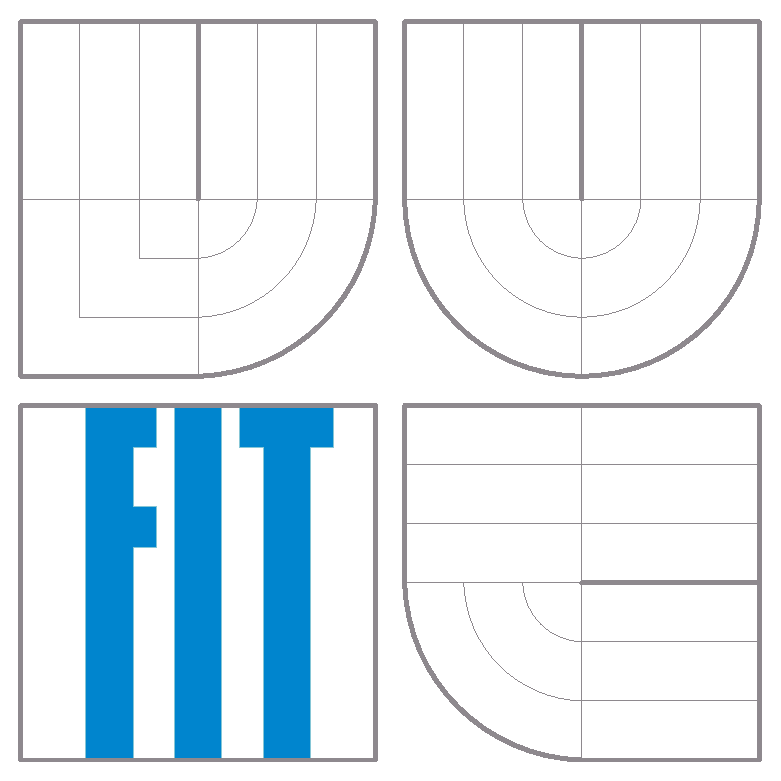
\includegraphics[height=9mm]{logo.eps} }
	\end{frame}

	
	%% -----------------------------
	
	% Goals
	% CUDA architecture and GPU
	% Waldboost, LBP and object detection
	% Implementation
	% Future work
	
	\begin{frame}[t,fragile]
		\frametitle{Goals and contributions of the thesis}
		
		\begin{itemize}
			\item CUDA implementation of an object detector (waldboost+lbp) working real-time on videos (~25fps 1080p)
			\item Comparative measurements of GPU and CPU versions, GPU optimization research, measurements and discussion
		\end{itemize}		
		
	\end{frame}

	%% ------------------------------	

	\begin{frame}[t,fragile]
		\frametitle{NVIDIA CUDA}
		
	\begin{columns}[onlytextwidth]
		\begin{column}{0.7\textwidth}
		    \begin{itemize}
				\item GPGPU \textit{(General-purpose computing on graphics processor units)} technology
				\item similar to: OpenCL, C++ AMP, OpenGL compute shaders, DirectCompute
				\item extension to C/C++ (CUDA C) - uses its own compiler NVCC
				\item massive parallelism
				\item scientific calculations (chemistry, bioinformatics, \dots), computer vision \& imaging, medical imaging, weather, numerical analytics
			\end{itemize}
		\end{column}

		\begin{column}{0.3\textwidth}
			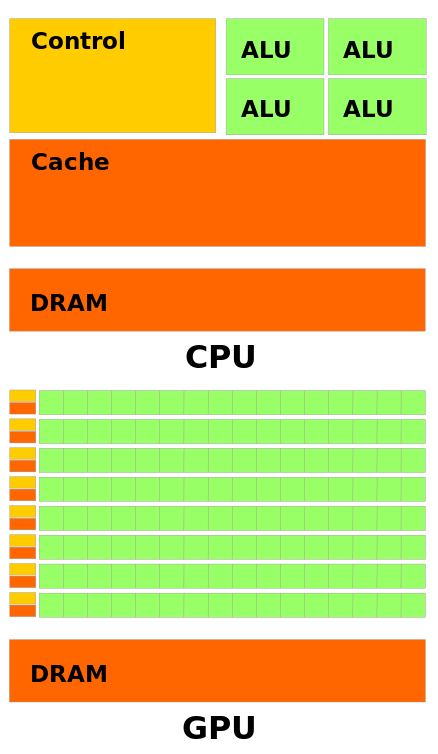
\includegraphics[width=\textwidth]{img/cpu-gpu.png}
		\end{column}
	\end{columns}				
			
	\end{frame}
	
	%% --------------------------
	
		\begin{frame}[t,fragile]
		\frametitle{Object detection}
		
		\begin{itemize}
			\item detecting specific objects of a certain class in digital images or videos
			\item \textbf{WaldBoost} - meta-algorithm, which sequentially processes a sample and discards when accumulated response reaches certain threshold
			\item \textbf{LBP} \textit{(Local Binary Pattern)} - feature to describe properties of an image
		\end{itemize}		
		
		\vspace{6mm}		
		
		\centering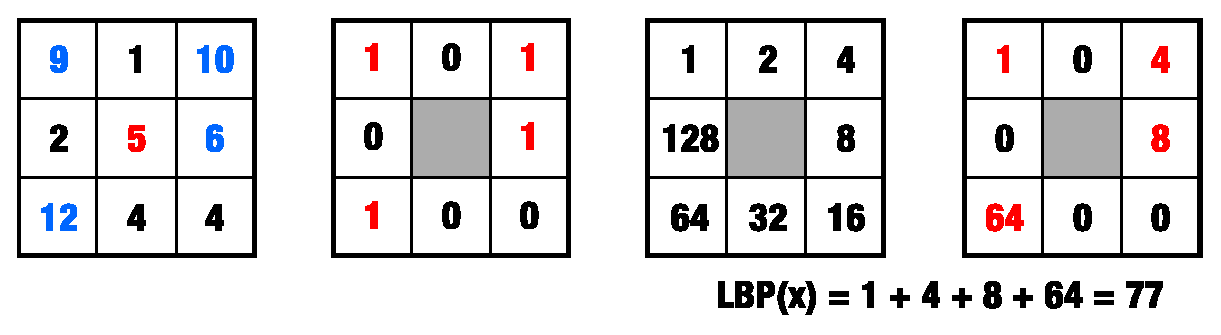
\includegraphics[width=0.8\textwidth]{img/lbp.eps}
		
	\end{frame}

	%% ------------------------------

	\begin{frame}[t,fragile]
	\frametitle{Implementation}					
	\begin{columns}[onlytextwidth]
		\begin{column}{0.45\textwidth}
			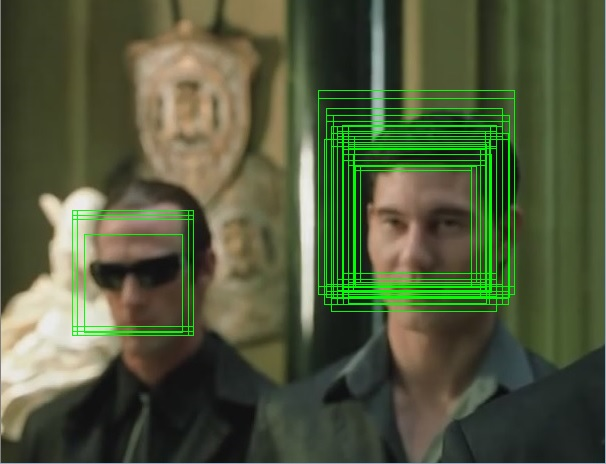
\includegraphics[width=\textwidth]{img/detections.jpg}
		\end{column}	
	
		\begin{column}{0.5\textwidth}
		    \begin{itemize}
				\item GPU and CPU implementation
				\item GPU version \\ (NVIDIA Quadro K1000M): 
				\\ \textbf{25 ms} (pyramidal image)
				\\ \textbf{60-100 ms} (detection)
				\\ \textbf{10 FPS} (HD video)

			\end{itemize}
		\end{column}	
	\end{columns}		

	\begin{small}
		\vspace{5mm}
		\centering\url{https://github.com/mmaci/vutbr-fit-object-detection}	
	\end{small}	
	\end{frame}
	
	%% ------------------------------

	\begin{frame}[t,fragile]
	\frametitle{Optimizations}					
	\begin{columns}[onlytextwidth]				
		\begin{column}{0.60\textwidth}
		    \begin{itemize}
				\item Bilinear interpolation using texture memory used for pyramidal image
				\item LBP features are 2x1, 1x2 and 2x2 - pyramidal image stored in texture memory and LBP computed using bilinear interpolation
			\end{itemize}
		\end{column}
		
		\begin{column}{0.35\textwidth}
			\includegraphics[width=\textwidth]{img/pipeline.eps}
		\end{column}	

	\end{columns}		
	\end{frame}
	
	%% --------------------------
	
	\begin{frame}[t,fragile]
	\frametitle{Future work}	
				
	\begin{itemize}
		\item thread rearrangement
		\item Lanczos interpolation
		\item pyramidal build optimization + mipmaps
		\item CPU and GPU measurements
	\end{itemize}				
						
	\end{frame}		
	
	%% --------------------------
	
	%% --------------------------
	
	\begin{frame}[t,fragile]
	\vspace{33mm}	
	\begin{Large}
	\begin{center}
		 Thank you for attention.
	\end{center}
	\end{Large}				
						
	\end{frame}

\end{document} 
